\subsection{Discussion of results}
\label{sec:DiscussionResults}
The perfect classification of goalkeepers can be justified by strength and weaknesses of these football positions.

 Goalkeepers have low values regarding sliding tackle, skill moves, sprint speed, etc. A visualization in a coordination systems \ref{fig:VisualAttributes} shows that goalkeepers (black) have the biggest deficits in these and other attributes (values in the bottom left corner). Defenders (blue) are better in these categories than goalkeepers. While midfielder (green) and strikers (orange) have nearly same strengths (one dot on top of each other in middle and top right corner). 

\begin{figure}
\centering
  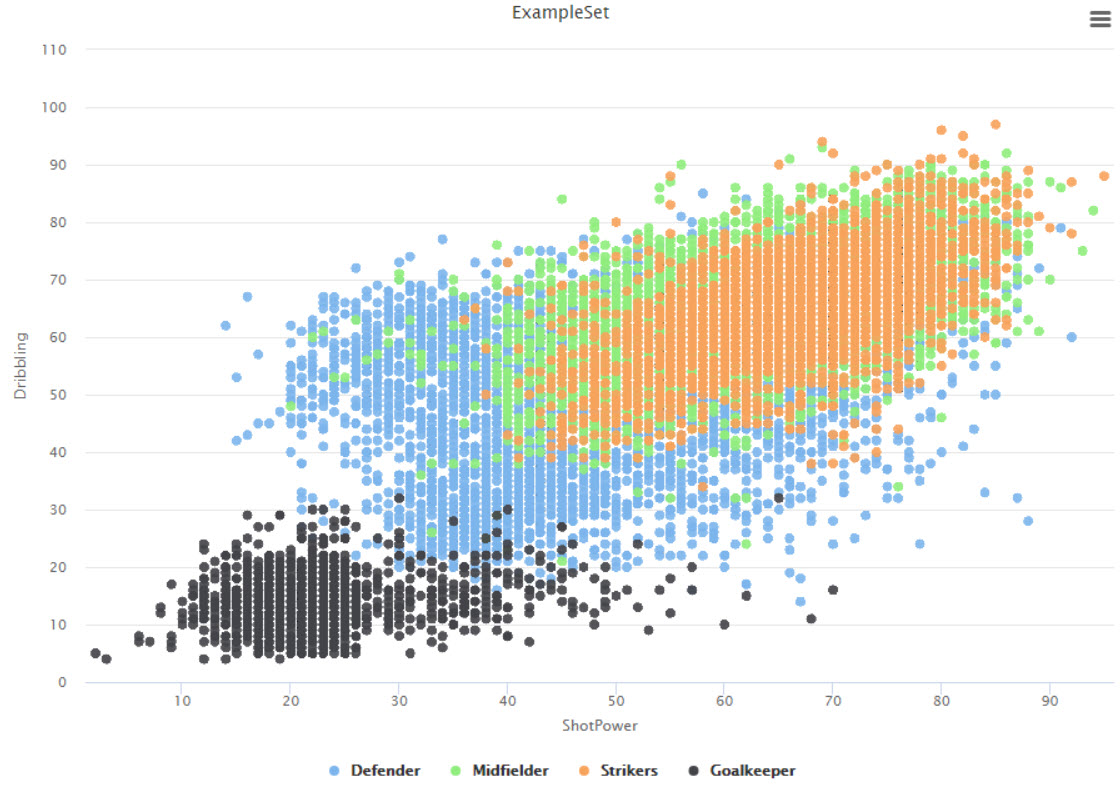
\includegraphics[width=8cm]{VisualizationAttributes.jpg}
  \caption{Visualization of two characteristics: dribbling and shot power}
  \label{fig:VisualAttributes}
\end{figure}

The result matches the expectations as the boundaries between strikers and midfielders are blurry. These two attributes are only an excerpt from more than 80 attributes but are typical for the data set.

As a conclusion, the data model to predict a soccer players position scores good result on the training and test data sets. Due to nearly identical attribute values for midfielders and strikers the accuracy decreased.